\documentclass[11pt,a4]{article}
%This makes the margins little smaller than the default
\usepackage{fullpage}

\oddsidemargin-0.3cm

\pagestyle{plain}

\usepackage{enumerate}
\usepackage{parskip}
\usepackage{listings}
\usepackage{hyperref}
\usepackage[pdftex]{graphicx}
\usepackage{placeins}
\usepackage{amsmath}

\graphicspath{{project1/_report/}}


\title{
        Computational Photography \linebreak Autumn Semester 2014 \linebreak
        \bf{Project 1}
}
\author{
        Laura Rettig\footnote{laura.rettig@unifr.ch}
       }
\date{\normalsize \today}

%-----------------------------------
\begin{document}
%-----------------------------------

\maketitle

\section{Spanish Castle Illusion}

This illusion works due to the so-called opponent process. This theory states that the visual system records differences between the antagonistic channels red and green as well as blue and yellow. Fixating on the inverse image for a while makes the cones ``tired'', i.e. the receptors in this area will become less reactive. When then switching to the neutral grey image, the antagonist will react more strongly. Therefore what was previously red in the inverse image will then be seen as green. \footnote{\url{http://en.wikipedia.org/wiki/Opponent_process}}

\begin{figure}[htb]
    \begin{center}
    	\includegraphics[width=300px]{1_grey.png}
        \caption{Grey image (from Y channel).}
    \end{center}
\end{figure}
\begin{figure}[htb]
    \begin{center}
        \includegraphics[width=300px]{1_inverted.png}
        \caption{Inverted RGB image.}
    \end{center}
\end{figure}

\newpage
\FloatBarrier
\section{Processing RAW Images}

\subsection{Bayer Demosaicing using Bilinear Filtering}

\begin{figure}[htb]
    \begin{center}
    	\includegraphics[width=300px]{21_given_grey.png}
    	\includegraphics[width=300px]{21_given_rec.png}
        \caption{Greyscale image of the input, and reconstructed to an RGB image.}
    \end{center}
\end{figure}
\FloatBarrier

I also tried this on an image of my own, captured in Canon's RAW CR2 format with a Canon PowerShot G15. I converted the input to tiff using the \texttt{dcraw} command:\\
\texttt{dcraw -c -w -o 0 -D "input.cr2" > "output.tiff"}

Since this image has 8 bit precision, I divided the values by 255 instead of 4096.

\begin{figure}[htb]
    \begin{center}
    	\includegraphics[width=350px]{21_own_grey.png}
        \includegraphics[trim = 50px 1930px 3610px 910px, clip, width=300px]{21_own_grey.png}
        \caption{Own image: Greyscale image of the input (with Bayer pattern). The ``grid'' can be easily detected.}
    \end{center}
\end{figure}

\begin{figure}[htb]
    \begin{center}
    	\includegraphics[width=350px]{21_own_reconstructed.png}
        \includegraphics[trim = 50px 1930px 3610px 910px, clip, width=300px]{21_own_reconstructed.png}
        \caption{Own image: Reconstructed to an RGB image (as mentioned in the slides, not standard RGB and no gamma correction).}
    \end{center}
\end{figure}

\newpage
\FloatBarrier
\subsection{Median Filter Demosaicing}

\begin{figure}[htb]
    \begin{center}
    	\includegraphics[width=200px]{22_unfiltered.png}
        \includegraphics[width=200px]{22_filtered.png}
        \caption{The image \texttt{black and white raw.tif}, on the left after Bayer demosaicing with bilinear filter (clearly visible artifacts), on the right after Median filtering the left image. Artifacts have been mostly removed, although the filter is not perfect. \label{img:22whole}}
    \end{center}
\end{figure}

\begin{figure}[htb]
    \begin{center}
    	\includegraphics[trim = 210px 450px 220px 0px, clip, width=180px]{22_unfiltered.png}
        \includegraphics[trim = 210px 450px 220px 0px, clip, width=180px]{22_filtered.png}
        \caption{Zooming in to the edge makes highlights the difference. While we have strong color fringing on the left, in the right (filtered) image only very little remains, hardly visible on normal scale. \label{img:22zoom}}
    \end{center}
\end{figure}

Applying the median filter to the U and V channels (essentially, these are very close to the color differences between B-G and R-G) normalizes unusual peaks which have resulted from bilinear interpolation at the edges due to extreme values in one direction or the other.

Interestingly enough, changing the size of the median filter (utilized here 5x5) doesn't change the output. This would probably be different on a different image, where there isn't just one hard cut, but more in the surroundings (e.g. the example image seen in the lecture).


\newpage
\FloatBarrier
\subsection{Color Balancing}
\begin{figure}[htb]
    \begin{center}
    	\includegraphics[width=275px]{23_bernBlaustich.jpg}
        \includegraphics[width=275px]{23_autocolor1.jpg}
        \includegraphics[width=275px]{23_mancolor1.jpg}
        \caption{The original image (overly blue), after automatic color balancing, and after manual white balance. \label{img:color1}}
    \end{center}
\end{figure}

\begin{figure}[htb]
    \begin{center}
    	\includegraphics[width=270px]{23_IMG_1558.JPG}
        \includegraphics[width=270px]{23_autocolor2.jpg}
        \includegraphics[width=270px]{23_mancolor2.jpg}
        \caption{The original image under a very strong red light, after automatic color balancing, and after manual white balance. \label{img:color2}}
    \end{center}
\end{figure}

\begin{figure}[htb]
    \begin{center}
    	\includegraphics[width=275px]{23_IMG_4977.jpg}
        \includegraphics[width=275px]{23_autocolor3.jpg}
        \includegraphics[width=275px]{23_mancolor3.jpg}
        \caption{The original image (too yellow due to the interior lighting), after automatic color balancing, and after manual white balance. \label{img:color3}}
    \end{center}
\end{figure}

In Figure~\ref{img:color1}, we can see that the automatic variant works very well and the image appears correct. For the manual color correction, a pixel in the shady areas of the background mountains was chosen. This yields a lighter correction. This pixel quite possibly isn't ``supposed'' to be grey, but have a slight tint to yellow from the overly lighting of the scenery. The pixel itself may be on a grey object, but be reflecting some colored object, leading to an incorrect balancing.

Figure~\ref{img:color2} was taken in a room that was entirely illuminated with a strong red light. Automatic color correction adjusts the colors too strongly in the opposite direction, white/grey areas becoming overly blue-green. Since this image is naturally stronger on the red side with the predominant red walls, the grey world assumption is incorrect here. Manual color correction works well when an appropriate input pixel is chosen. To produce the output here, a pixel in the left white map area was chosen. The correction leaves the fact intact that the scene is reddish, but corrects the grey pixels. \\
Another challenge with this image was choosing a good pixel: since the room was very dark, the image was taken with a high ISO. This has made it noisy, and noisy pixels differ from what would be in that area.

Similarly in Figure~\ref{img:color3}, while both color balancing methods work fairly well, the automatic adjustment is slightly too strong, so that grey areas, such as the floor, appear purple/blue (due to an incorrect grey world assumption, as in the previous figure). For the manual correction, a pixel on the floor was chosen which is supposed to be grey. The glass roof, on the other hand, was covered with snow when the image was taken, so the original image seems correct for this. There is a strong yellow light indoors, which does not shine towards the roof. Color balancing, especially the manual way, does a good job at correcting the colors for the indoors objects, while the roof becomes too blue. Since not all parts of the scene are under the same yellow light, global color balancing (manual and automatic) might not be a good strategy here. This can be generally said for images: If there are differences in the illumination of the pictured scene, a global correction can't be correct for all parts. Color constancy in human perception, on the other hand, has no problem detecting different light at different objects and adjusting accordingly.

\newpage
\FloatBarrier
\subsection{Global Contrast Adjustment}

\begin{figure}[htb]
    \begin{center}
    	\includegraphics[height=160px]{24_gamma1_before.jpg}\\
        \includegraphics[height=150px]{24_linear1.jpg}
        \includegraphics[height=200px]{24_linear1_plot.png}\\
        \includegraphics[height=150px]{24_gamma1.jpg}
        \includegraphics[height=200px]{24_gamma1_plot.png}
        \caption{Image before, with linear scaling to [0.1, 0.8], with gamma correction of 2.2, and the corresponding plots.}
    \end{center}
\end{figure}


\begin{figure}[htb]
    \begin{center}
    	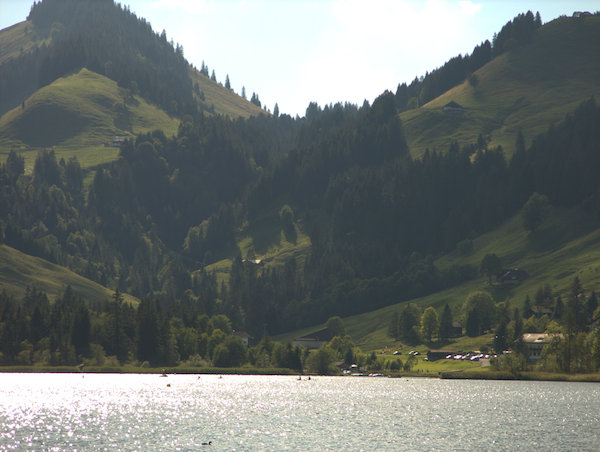
\includegraphics[height=160px]{24_schwarzsee.jpg}\\
        \includegraphics[height=150px]{24_linear2.jpg}
        \includegraphics[height=200px]{24_linear2_plot.png}\\
        \includegraphics[height=150px]{24_gamma2.jpg}
        \includegraphics[height=200px]{24_gamma2_plot.png}
        \caption{Image before, with linear scaling to [0.2, 0.9], with gamma correction of 1.5, and the corresponding plots.}
    \end{center}
\end{figure}

\begin{figure}[htb]
    \begin{center}
    	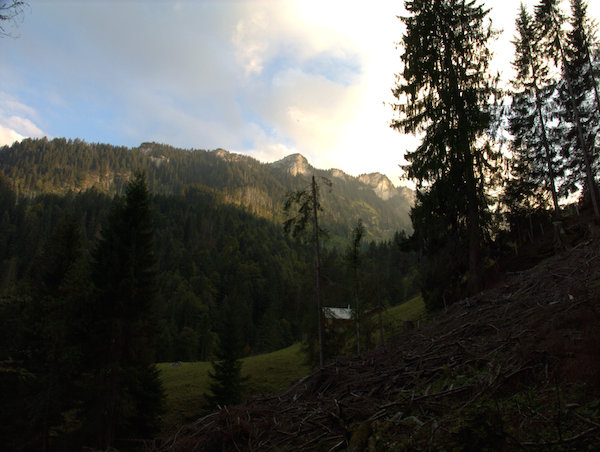
\includegraphics[height=160px]{24_schwarzsee2.jpg}\\
        \includegraphics[height=150px]{24_linear3.jpg}
        \includegraphics[height=200px]{24_linear3_plot.png}\\
        \includegraphics[height=150px]{24_gamma3.jpg}
        \includegraphics[height=200px]{24_gamma3_plot.png}
        \caption{Image before, with linear scaling to [0, 0.75], with gamma correction of 0.67, and the corresponding plots.}
    \end{center}
\end{figure}

\newpage
\FloatBarrier
\section{Bonus}

I performed automatic color balancing on the image that I had used in 2.2, a gamma transformation with $\gamma = 0.67$, and a linear contrast scaling to a range of $[0.2,1]$. The output can be seen in Figure~\ref{img:bonus}.

\begin{figure}[htb]
    \begin{center}
        \includegraphics[width=400px]{3_IMG_0871.jpg}
        \caption{Image with improved RAW processing.\label{img:bonus}}
    \end{center}
\end{figure}

I obtained the transformation matrix for the Canon PowerShot G15 from the \texttt{trans$[]$} in \texttt{table$[]$} in the class \texttt{adobe\_coeff}, divided by 10000:\\
$\begin{matrix}
       0.7474 & -0.2301 & -0.0567           \\
       -0.4056 & 1.1456           & 0.2975 \\
       -0.0222         & 0.0716 & 0.4181
\end{matrix}$

But this made the image even greener, and applying other matrices (namely \texttt{xyzd50\_srgb} or \texttt{adobe\_rgb}) did not make it better. So I did not succeed in the color correction.
%-------------------------
\end{document}
%-------------------------







